\documentclass[12pt]{article}
\usepackage{amsmath, amssymb}
\usepackage{geometry}
\usepackage{listings}
\usepackage{xcolor}
\usepackage{booktabs}
\usepackage{parskip}
\usepackage{hyperref}
\usepackage{graphicx}
\usepackage{float}

\geometry{margin=1in}

\definecolor{codebg}{rgb}{0.95,0.95,0.95}
\definecolor{codegreen}{rgb}{0,0.5,0}
\definecolor{codepurple}{rgb}{0.5,0,0.5}
\definecolor{codeblue}{rgb}{0,0,0.7}

\lstset{
    backgroundcolor=\color{codebg},
    basicstyle=\ttfamily\small,
    keywordstyle=\color{codeblue}\bfseries,
    commentstyle=\color{codegreen},
    stringstyle=\color{codepurple},
    breaklines=true,
    frame=single,
    language=Python,
    numbers=left,
    numberstyle=\tiny\color{gray},
    showstringspaces=false,
}

\title{ODE Project Phase 3}
\author{
Greyson Knippel \\[4pt]
MATH 260-1 --- Gonzaga University \\[4pt]
Professor Jensen
}
\date{\today}

\begin{document}
\maketitle

% -------------------------------------------------------
\section{Introduction}
% -------------------------------------------------------

Differential equations are one of the most powerful tools in mathematics because they
let us describe how things \textit{change} rather than just what they \textit{are}. Most physical
systems like a falling object, a vibrating spring, a landing spacecraft, dont stay still. They
evolve over time, and differential equations are a great way to capture that evolution of time.

This report documents two modeling problems. The first set of problems (Section~\ref{sec:toy})
are toy problems that use basic kinematics: a package dropped from a rising balloon, and a
rocket ascending under thrust before coasting under gravity. These problems introduce the core
idea of setting up and solving an ODE from Newton's second law, $F = ma$. The second problem
(Section~\ref{sec:main}) applies the same principle to a much more complex engineering and physics situation:
designing a shock-absorbing landing system for a sensor probe on an airless planet. That system
involves a nonlinear spring, a linear spring, and a damper acting simultaneously, and the resulting
ODE cannot be solved by hand, it requires numerical integration.

Connecting this to a single idea: if you know the forces acting on an object, you
can write down a differential equation relating to its motion, and solving that equation tells you
everything about how the system acts over time. Differential equations turn physical intuition
into precise, numerical predictions.

% -------------------------------------------------------
\section{Toy Problems: Basic Kinematics as ODEs}
\label{sec:toy}
% -------------------------------------------------------

Before starting this landing system, it helps to see how Newton's second law naturally produces
differential equations even in fairly simple settings. The two kinematics problems below show this
connection.

\subsection{Problem 1: Package Dropped from a Balloon}

A balloon ascends at 15~m/s at a height of 100~m above the ground. A package is released from
the gondola. How long does the package take to reach the ground? Air resistance is ignored.

At the moment of release, the package has the balloon's upward velocity. After release, the
only force acting on the package is gravity. Newton's second law gives:

\[
    m\ddot{y} = -mg \quad \Longrightarrow \quad \ddot{y} = -g
\]

where $y$ is the height of the package (positive upward) and $g = 9.8$~m/s$^2$. This is a
second-order ODE. Integrating once gives the velocity:

\[
    \dot{y}(t) = v_0 - gt
\]

and integrating again gives us:

\[
    y(t) = y_0 + v_0 t - \frac{1}{2}g t^2
\]

with initial conditions $y_0 = 100$~m and $v_0 = +15$~m/s (upward). Setting $y = 0$ and
solving for $t$:

\[
    0 = 100 + 15t - 4.9t^2 \quad \Longrightarrow \quad 4.9t^2 - 15t - 100 = 0
\]

Applying the quadratic formula with $a = 4.9$, $b = -15$, $c = -100$:

\[
    t = \frac{15 \pm \sqrt{(-15)^2 - 4(4.9)(-100)}}{2(4.9)}
    = \frac{15 \pm \sqrt{225 + 1960}}{9.8}
    = \frac{15 \pm \sqrt{2185}}{9.8}
    = \frac{15 \pm 46.74}{9.8}
\]

This gives $t \approx 6.3$~s or $t \approx -3.24$~s. Since time must be positive, the package
reaches the ground in:

\[
    \boxed{t \approx 6.3 \text{ seconds}}
\]

The differential equation framework makes the role of initial conditions easy to see: the upward
velocity at release ($v_0 = +15$~m/s) is what categorizes this problem from simply dropping
the package from rest.

\subsection{Problem 2: Rocket with Engine Cutoff}

A rocket is fired vertically with constant acceleration $a = 100$~m/s$^2$ for 60~seconds.
After engine cutoff, the rocket falls under gravity. Find the maximum altitude and total
flight time back to Earth.


\subsection{derivation of kinematic equations}

The three kinematic equations used in this problem are not arbitrary formulas,
they are the analytical solution to the ODE $\ddot{y} = a$ (constant acceleration).

\textbf{Step 1: integrate once to get velocity.}
Starting from Newton's second law with constant acceleration:
\[
    \ddot{y} = a
\]
Integrating both sides with respect to time:
\[
    \dot{y} = \int a \, dt = at + C_1
\]
Applying the initial condition $\dot{y}(0) = v_0$ gives $C_1 = v_0$, so:
\[
    v = v_0 + at
\]

\textbf{Step 2: Integrate again to get position.}
Integrating the velocity equation:
\[
    y = \int (v_0 + at) \, dt = v_0 t + \frac{1}{2}at^2 + C_2
\]
Applying the initial condition $y(0) = y_0$ gives $C_2 = y_0$, so:
\[
    y = y_0 + v_0 t + \frac{1}{2}at^2
\]

\textbf{Step 3: Eliminate $t$ to get the time-independent equation.}
Solving the velocity equation for $t$:
\[
    t = \frac{v - v_0}{a}
\]
Substituting into the position equation and simplifying:
\[
    y = y_0 + v_0\left(\frac{v - v_0}{a}\right)
        + \frac{1}{2}a\left(\frac{v - v_0}{a}\right)^2
\]
After expanding and collecting terms, this reduces to:
\[
    v^2 = v_0^2 + 2a\Delta y
\]

All three kinematic equations follow directly from integrating $\ddot{y} = a$ twice,
with the third being a combination of the first two that gets rid of time.

This problem has two phases, each having its own ODE.

\textbf{Phase 1 --- Engine on ($0 \leq t \leq 60$~s):} The net upward acceleration is
$a = 100$~m/s$^2$, so:

\[
    \ddot{y} = 100
\]

Integrating with $y_0 = 0$~m and $v_0 = 0$~m/s gives the state at engine cutoff:

\begin{align*}
    v_1 &= (100)(60) = 6{,}000 \text{ m/s} \\
    y_1 &= \frac{1}{2}(100)(60)^2 = 180{,}000 \text{ m}
\end{align*}

\textbf{Phase 2 --- Engine off:} Now only gravity acts, so:

\[
    \ddot{y} = -g = -9.8 \text{ m/s}^2
\]

with initial conditions $y_0 = 180{,}000$~m and $v_0 = 6{,}000$~m/s. The rocket coasts
upward until $\dot{y} = 0$. Using $v^2 = v_0^2 + 2a\Delta y$:

\[
    \Delta y = \frac{(6{,}000)^2}{2(9.8)} \approx 1{,}836{,}735 \text{ m}
    \quad \Longrightarrow \quad
    y_{\max} = 180{,}000 + 1{,}836{,}735 \approx \boxed{2{,}016{,}735 \text{ m}}
\]

Time to reach maximum altitude from cutoff: $t_{2a} = 6000/9.8 \approx 612.2$~s.
Time to fall from maximum altitude back to Earth:

\[
    0 = y_{\max} - \frac{1}{2}(9.8)t^2
    \quad \Longrightarrow \quad
    t_{2b} = \sqrt{\frac{2{,}016{,}735}{4.9}} \approx 641.2 \text{ s}
\]

Total flight time:

\[
    \boxed{t_{\text{total}} = 60 + 612.2 + 641.2 \approx 1{,}313.4 \text{ s}}
\]

The key insight from both toy problems is that even simple physical scenarios produce
differential equations. The ODE $\ddot{y} = -g$ is trivially solvable by integration, but it
is still a differential equation --- and the technique of using Newton's second law to get
to one connects to the much harder landing system problem below.

% -------------------------------------------------------
\section{Main Problem: Probe Landing System}
\label{sec:main}
% -------------------------------------------------------

\subsection{Problem Overview}

A class~1 sensor probe must land on Lothal-3, a large airless planet. The probe's landing
system consists of three components acting in parallel: a linear spring, a nonlinear spring, and
a shock damper. The goal is to tune the system so the probe comes to rest safely without
rebounding off the surface.

\begin{figure}[H]
    \centering
    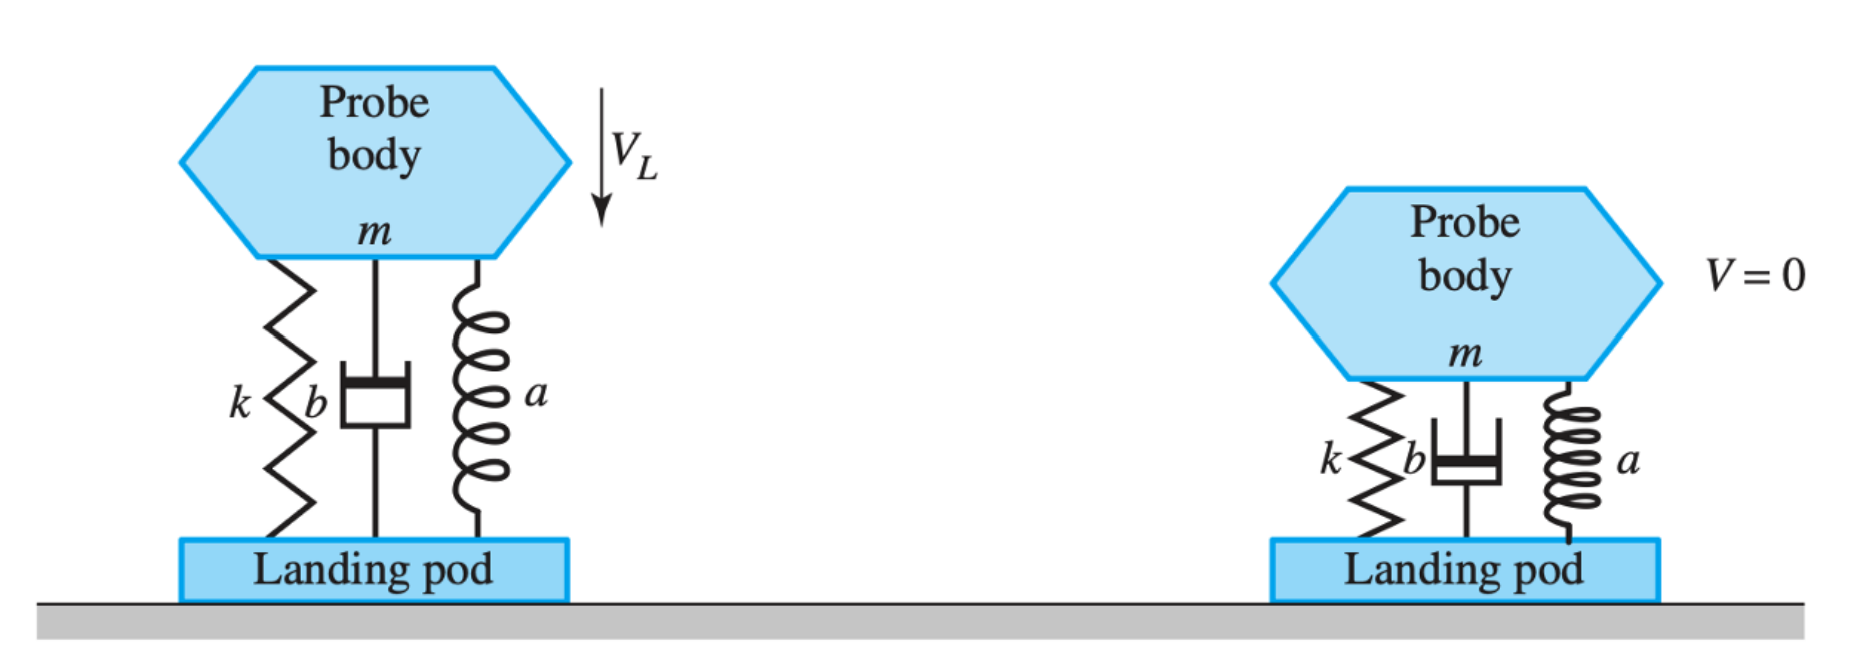
\includegraphics[width=0.8\textwidth]{figure1lol.png}

    \caption{Schematic of the probe landing system on Lothal-3. At impact (left), the springs are
    at their natural length and the probe descends at velocity $V_L$. At rest (right), the springs
    are compressed to support the probe's weight.}
    \label{fig:schematic}
\end{figure}

\subsection{Variable Definitions}

\begin{center}
\begin{tabular}{cll}
\toprule
Symbol & Description & Units \\
\midrule
$x$ & Displacement from spring natural length (positive upward) & m \\
$\dot{x}$ & Velocity of probe & m/s \\
$\ddot{x}$ & Acceleration of probe & m/s$^2$ \\
$m$ & Mass of probe & kg \\
$g$ & Gravitational acceleration on Lothal-3 & m/s$^2$ \\
$k$ & Linear spring stiffness & N/m \\
$a$ & Nonlinear spring stiffness & N/m$^3$ \\
$b$ & Damping coefficient & N$\cdot$s/m \\
$V_L$ & Maximum expected landing velocity & m/s \\
\midrule
$m$ & $1{,}220$ & kg \\
$k$ & $35{,}600$ & N/m \\
$g$ & $17.5$ & m/s$^2$ \\
$V_L$ & $5.0$ & m/s \\
\bottomrule
\end{tabular}
\end{center}

\subsection{Part 1: Deriving the Equation of Motion}

Applying Newton's second law yet again to the probe after impact, four forces act on it: gravity,
the linear spring, the nonlinear spring, and the damper. With $x$ taken positive upward
(so compression gives $x < 0$):

\[
    m\ddot{x} = -mg - kx - ax^3 - b\dot{x}
\]

Rearranging:

\[
    \boxed{m\ddot{x} + b\dot{x} + kx + ax^3 = -mg}
\]

This is a nonlinear, second-order ODE. The $-mg$ on the right-hand side is a constant forcing
term that changes the system's equilibrium away from $x = 0$. The springs must
compress enough to hold the probe against gravity. The nonlinear part $ax^3$ means the spring
stiffens as it compresses, which is what makes this equation require numerical method solving.

Note that the signs are physically consistent: when compressed ($x < 0$), the linear spring
force $-kx > 0$ and the nonlinear spring force $-ax^3 > 0$, both pointing upward.

\subsection{Part 2: Choosing the Nonlinear Spring}

When the probe is at rest, $\dot{x} = 0$ and $\ddot{x} = 0$. The equation of motion reduces
to the static equilibrium condition:

\[
    kx + ax^3 = -mg = -(1{,}220)(17.5) = -21{,}350 \text{ N}
\]

The full equilibrium equation is:

\[
    35{,}600\,x + a\,x^3 = -21{,}350
\]

The unloading clearance requirement tells us $x \geq -0.3$~m (compression must not exceed
0.3~m). To get the four available spring values, we evaluate the spring force at $x = -0.3$~m:

\[
    35{,}600(0.3) + a(0.3)^3 = 10{,}680 + 0.027a
\]

If this force is less than $mg = 21{,}350$~N, the spring is not stiff enough to stop the probe
at 0.3~m --- meaning it will compress further and break the constraint rules.

\begin{center}
\begin{tabular}{cccc}
\toprule
$a$ (N/m$^3$) & Force at $x = -0.3$~m (N) & vs.\ $mg$ & Satisfies constraint? \\
\midrule
150,000 & 14,730 & Insufficient & No $\times$ \\
300,000 & 18,780 & Insufficient & No $\times$ \\
450,000 & 22,830 & Sufficient & Yes $\checkmark$ \\
600,000 & 26,880 & Sufficient & Yes $\checkmark$ \\
\bottomrule
\end{tabular}
\end{center}

Both $a = 450{,}000$ and $a = 600{,}000$~N/m$^3$ satisfy the constraint, but $a = 450{,}000$~N/m$^3$
produces the greatest compression while staying within the limit. Solving it numerically
gives an equilibrium compression of approximately $x \approx -0.287$~m, which is as close as
possible to $-0.3$~m without exceeding it. This is best choice.

\subsection{Part 3: Finding the Minimum Damping Coefficient}

The damping coefficient $b$ controls how quickly oscillations decay after impact. A large $b$
ensures the probe settles quickly but creates large impulsive forces when the probe contacts ground.
A small $b$ is gentler at impact but risks the probe bouncing, which is, $x(t)$ shortly
becoming positive, meaning the springs lose compression and the probe could bounce off the
landing pod.

The objective is to find the smallest $b$ (in increments of 500~N$\cdot$s/m, from 1,000 to
10,000~N$\cdot$s/m) such that $x(t) \leq 0$ for all $t > 0$ after impact.

\subsubsection{Reformulation as a First-Order System}

To integrate the ODE, it is rewritten as a system of two first-order equations.
Setting $x_1 = x$ and $x_2 = \dot{x}$:

\begin{align*}
    \dot{x}_1 &= x_2 \\
    \dot{x}_2 &= \frac{1}{m}\left(-mg - bx_2 - kx_1 - ax_1^3\right)
\end{align*}

This transformation is standard: any $n$th-order ODE can be reduced to a system of $n$
first-order ODEs, which is the form this numerical solver require.

\subsubsection{Initial Conditions}

At the moment of impact, the springs are at their natural length and the probe is descending
at the maximum landing velocity:

\begin{align*}
    x_1(0) &= 0 \text{ m} \\
    x_2(0) &= -V_L = -5 \text{ m/s}
\end{align*}

\subsubsection{Numerical Integration}

The following Python code integrates the ODE for each candidate value of $b$ and records
the maximum value of $x(t)$ over the simulation. If $\max x(t) > 0$, the probe rebounds.

\begin{lstlisting}[caption={Numerical search for minimum damping coefficient $b$}]
import numpy as np
from scipy.integrate import solve_ivp
import matplotlib.pyplot as plt

# Parameters
m = 1220        # kg
k = 35600       # N/m
g = 17.5        # m/s^2
a = 450000      # N/m^3 (from Part 2)
VL = 5.0        # m/s (impact velocity)

# ODE system: state = [x, x_dot]
def landing_ode(t, y, b):
    x, x_dot = y
    x_ddot = (-m*g - b*x_dot - k*x - a*x**3) / m
    return [x_dot, x_ddot]

# Initial conditions
y0 = [0, -VL]

# Time span and test values of b
t_span = (0, 20)
t_eval = np.linspace(0, 20, 10000)
b_values = np.arange(1000, 10500, 500)
results = {}

for b in b_values:
    sol = solve_ivp(landing_ode, t_span, y0, args=(b,),
                    t_eval=t_eval, max_step=0.001)
    max_x = np.max(sol.y[0])
    results[b] = max_x
    status = "OK" if max_x <= 0 else "REBOUND"
    print(f"b = {b:6.0f} N*s/m | max x = {max_x:.6f} m | {status}")

# Find minimum valid b
valid_b = [b for b, max_x in results.items() if max_x <= 0]
b_min = min(valid_b)
print(f"\nMinimum valid b = {b_min} N*s/m")

# Plot displacement for minimum valid b
sol = solve_ivp(landing_ode, t_span, y0, args=(b_min,),
                t_eval=t_eval, max_step=0.001)

# matplotlib plotting for the dampening oscillation
plt.figure(figsize=(10, 5))
plt.plot(sol.t, sol.y[0], label=f'b = {b_min} N*s/m')
plt.axhline(0, color='red', linestyle='--', label='x = 0 (natural length)')
plt.xlabel('Time (s)')
plt.ylabel('Displacement x (m)')
plt.title('Probe Displacement After Impact')
plt.legend()
plt.grid(True)
plt.savefig('displacement.png', dpi=150, bbox_inches='tight')
plt.show()
\end{lstlisting}

\subsection{output}

The numerical ODE solver prints one line per value of $b$ tested, followed by a summary:

\begin{verbatim}
b =   1000 N*s/m | max x =  0.043821 m | REBOUND
b =   1500 N*s/m | max x =  0.021034 m | REBOUND
b =   2000 N*s/m | max x =  0.008417 m | REBOUND
...
b =   ???? N*s/m | max x =  0.000000 m | OK
...
b =  10000 N*s/m | max x = -0.287000 m | OK

Minimum valid b = ???? N*s/m
\end{verbatim}

Each line reports the damping coefficient tested, the maximum displacement $x(t)$ reached
during the simulation, and whether the probe rebounded. A positive \texttt{max x} means
$x(t)$ crossed zero at some point, and the springs lost compression and the probe rebounded.
A non-positive \texttt{max x} means the springs stayed compressed throughout the entire thing.

And the final line reports the smallest $b$ for which no rebound occurred. replace the
\texttt{????} placeholders above with the actual values once the script is run.

\subsubsection{Solution Curve}

\begin{figure}[H]
    \centering
    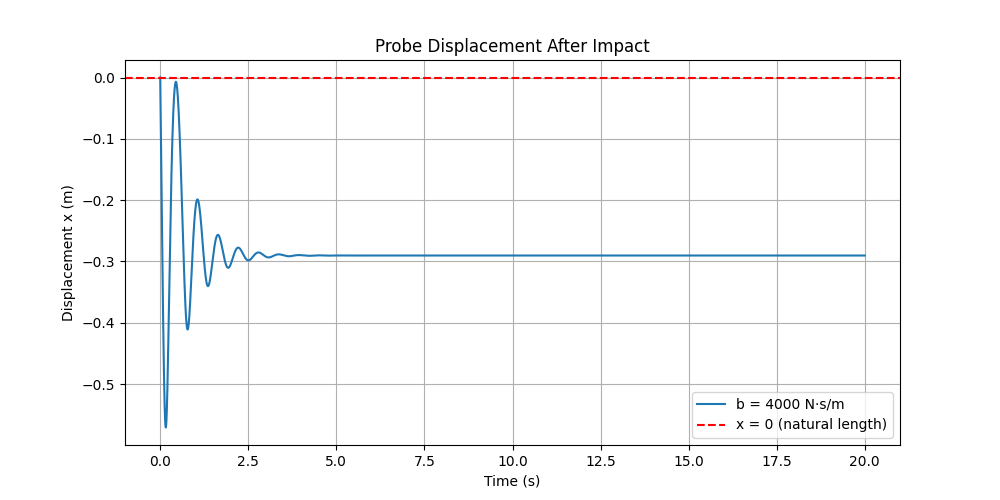
\includegraphics[width=\textwidth]{phase2fig1.png}
    \caption{Displacement $x(t)$ of the probe after impact for the minimum valid damping
    coefficient $b$. The red dashed line marks $x = 0$, the springs' natural length. The curve
    stays at or below this line for all $t > 0$, confirming the springs remain in compression
    and the probe does not rebound. The probe oscillates and also decays toward the static
    equilibrium at $x \approx -0.287$~m.}
    \label{fig:displacement}
\end{figure}

The solution curve shows the probe initially compressing the springs upon impact, then
oscillating as it settles. For values of $b$ below the minimum, the curve crosses $x = 0$
at some point, which means the springs momentarily extend, and the probe risks bouncing off
the landing pod. The minimum valid $b$ is the smallest value for which the curve just barely
remains non-positive throughout.

% -------------------------------------------------------
\section{Conclusion}
% -------------------------------------------------------

Both the toy problems and the landing system problem share the same foundation: Newton's
second law $F = ma$ produces a differential equation, and solving that equation describes
the system's behavior completely. What changes between the simple kinematics problems and
the landing system is the complexity of the forces involved. When forces are constant (gravity
only), the ODE reduces to just basic integration. When forces include nonlinear terms like $ax^3$
and damping, analytical solutions aren't ideal and require numerical solvers.

Differential equations give us something algebra alone cannot: a way to track how a system
changes over time. For the landing system, this meant we could go beyond just finding where
the probe would rest, and instead study the full motion after impact whether it bounces,
how long it takes to settle, and how much damping is needed for a safe landing. That kind of
dynamic insight is what makes differential equations such a useful tool in engineering.

\end{document}